\documentclass[12pt, letterpaper]{article}
\usepackage{graphicx}
\usepackage{amsmath}
\usepackage{amssymb}
\usepackage{float}
\graphicspath{{images/}}
\title{Summary of Gradient descent and Newton's method from coursera course}
\author{Evert Jan Karman\thanks{Inspired by coursera mathematics for ML specialization.}}
\date{October 2025}
\begin{document}
\maketitle

In this document we provide brief summary of how coursera explains
\begin{itemize}
    \item Gradient descent with one variable
    \item Gradient descent with two or more variables
    \item Newton's method with one variable
    \item Newton's method with two or more variables
\end{itemize}

\section{Gradient descent with one variable}

Assume that we have a continuous function f defined on $\mathbb{R}$:

\begin{figure}[H]
    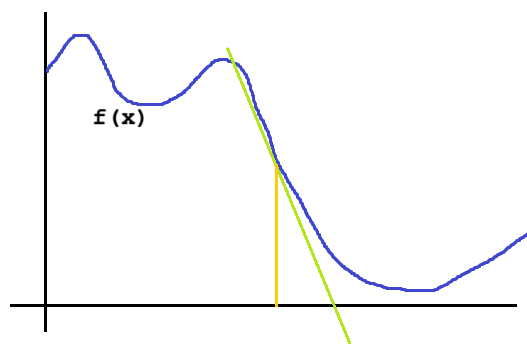
\includegraphics{fx_example_01.png}
\end{figure}
Assume that f is also differentiable with derivative $f'(x)$.\\
We also have a starting point $x_0$.\\
Then we get $x_1$ by subtracting $f'(x_0) \cdot \alpha$ from x, where $\alpha$ is called the learning rate, which we can choose before doing this procedure.\\
Usual values for $\alpha$ are $0.01$ or $0.05$.\\
We iterate this, so that we get an array which is recursively defined as:\\
\[x_{k+1} = x_k - f'(x_k) \cdot \alpha\]

This array will converge to the minimum of f.
The pitchfalls here are, that the procedure may end in a local minimum, while f has a stronger minimum elsewhere.\\
Or with a less than optimal choice for the learning rate, the array could even diverge.

\section{Gradient descent with two or more variables}
With a function $f(x, y)$ of more variables, we can determine the gradient:
\[
\nabla f(x,y) = \left( \frac{\partial f}{\partial x}, \frac{\partial f}{\partial y} \right)
\]
The method is the same, but where we took the derivative for one variable, we will now take the gradient, and the recursive definition of our array  $(x_k,y_k)$ becomes:\\
\[(x_{k+1},y_{k+1}) = (x_k,y_k) - \nabla f(x,y) \cdot \alpha\]


\section{Newton's method with one variable}
Newton's method finds the zeroes of a function f. Because we're interested in finding a minimum of f,
Newton's method will help us find the zero of it's derivative $f'$.\\
\\
\begin{figure}[H]
    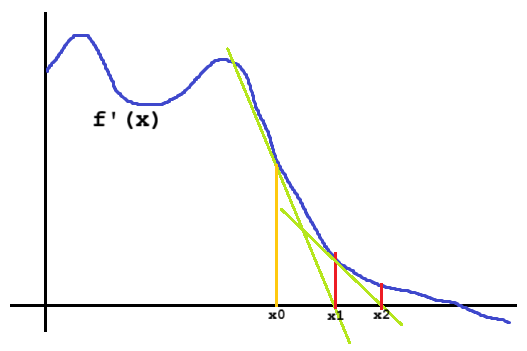
\includegraphics{fx_example_02.png}
\end{figure}
Geometrically, when you have the graph of f, and you have a starting point $x_0$, we start by drawing the tangent line.\\
Then we see where this tangent line intersects with the x-axis. That will be $x_1$.\\
By iterating this procedure we get an array $(x_k)_{k=0,1,\ldots}$.

From the geometrical aspect of the procedure, we can give a formula between $x_{k+1}$ and $x_k$:
\[
x_{k+1} = x_k - (f'(x_k) / f''(x_k))
\]
(that is for finding the zero of $f'$)
The idea is that the array $(x_k)$ converges to the value x where $f'(x) = 0$.\\

In order to know if $f'(x)$ points to a minimum of f, we need to look at the second derivative $f''(x)$:\\
$f''(x) > 0 \Rightarrow$ f has a minimum at x\\
$f''(x) < 0 \Rightarrow$ f has a maximum at x\\
$f''(x) = 0 \Rightarrow$ inconclusive, perhaps an inflection point\\


\section{Newton's method with two or more variables}
Say we have function $f(x,y)$ of 2 variables.\\

Then here we have it's Hessian matrix:
\[
H_f(x,y) =
\begin{pmatrix}
\frac{\partial^2 f}{\partial x^2} & \frac{\partial^2 f}{\partial x \partial y} \\[1em]
\frac{\partial^2 f}{\partial y \partial x} & \frac{\partial^2 f}{\partial y^2}
\end{pmatrix}.
\]
Now at a given point (x,y) we'll calculate it's eigenvalues $\lambda_1, \lambda_2, \ldots$\\
(A 2 by 2 matrix would have at most two eigenvalues)\\

If the gradient has value (0,0) at point (x,y) then:
\begin{itemize}
    \item If all the eigenvalues of $H_f$ at (x,y) are positive, it's a minimum
    \item If all the eigenvalues of $H_f$ at (x,y) are negative, it's a maximum
    \item In other cases, it's inconclusive
\end{itemize}

In Newton's method generalized to more than one variables, the formula for the next point is:\\
\[
(x_{k+1},y_{k+1}) = (x_k,y_k) - ( H_f^{-1}(x_k,y_k) \cdot \nabla f(x_k,y_k) )
\]

\section{Example of a function of two variables}
We will look at this function:
\[
f(x,y) = 85 - \frac{1}{90}x^2(x-6)y^2(y-6)
\]
\begin{figure}[H]
    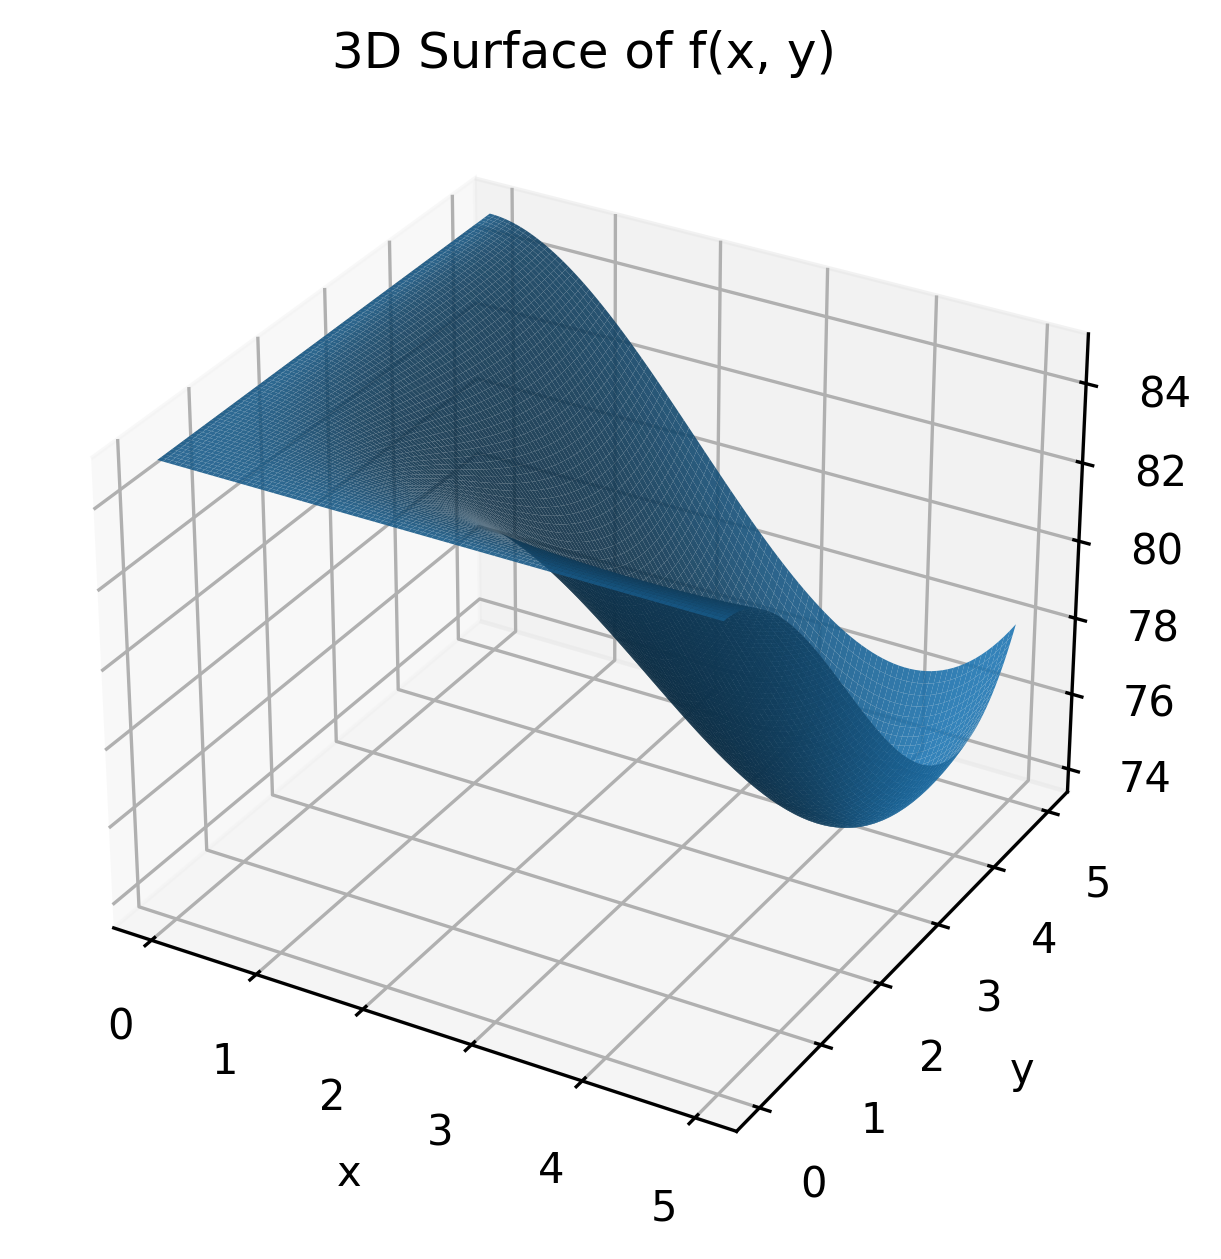
\includegraphics{3D_plot.png}
\end{figure}
Visually we see a possible minimum near point $(x,y) = (4,4)$.
We'll take $(x_0,y_0) = (1,1)$ and $\alpha = 0.01$ and from there, carry out gradient descent as actual example.\\

For gradient descent, we know that we need the formula for the gradient:
\[
\nabla f(x,y) = \left( - \frac{1}{90}(3x^2-12x)y^2(y-6), - \frac{1}{90}x^2(x-6)(3y^2-12y) \right)
\]
When we fill in x=1 and y=1 we calculate a gradient of (-0.5, -0.5).\\
We subtract this, multiplied by the learning rate, from (0, 0) and go to the next iteration.\\
Here we continued with a Python script that produced the following output:\\

{\footnotesize
\begin{verbatim}
0. x 1 y 1 --> (-0.500000000000000,-0.500000000000000)
1. x 1.00500000000000 y 1.00500000000000 --> (-0.506184974895937,-0.506184974895937)
2. x 1.01006184974896 y 1.01006184974896 --> (-0.512483652519824,-0.512483652519824)
3. x 1.01518668627416 y 1.01518668627416 --> (-0.518898669704649,-0.518898669704649)
...
510. x 3.99999989719588 y 3.99999989719588 --> (-4.38630910259973E-7,-4.38630910259974E-7)
511. x 3.99999990158219 y 3.99999990158219 --> (-4.19915991756169E-7,-4.19915991756170E-7)
512. x 3.99999990578135 y 3.99999990578135 --> (-4.01999575849742E-7,-4.01999575849743E-7)
513. x 3.99999990980134 y 3.99999990980134 --> (-3.84847593792869E-7,-3.84847593792870E-7)
\end{verbatim}
}
We see (x,y) approach (4,4) and we see the gradient approach (0,0). It takes 513 iterations.
We also tried learning rate 0.05. Then we saw the same behaviour, but only 104 iterations.

Now we will try to find the minimum using Newton's method. For this we need the second order derivatives:\\
\[
\frac{\partial^2 f}{\partial x^2} = - \frac{1}{90}(6x-12)y^2(y-6)
\]
\[
\frac{\partial^2 f}{\partial x \partial y} = - \frac{1}{90}(3x^2-12x)(3y^2-12y)
\]
\[
\frac{\partial^2 f}{\partial y \partial x} = - \frac{1}{90}(3x^2-12x)(3y^2-12y)
\]
\[
\frac{\partial^2 f}{\partial y^2} = - \frac{1}{90}x^2(x-6)(6y-12)
\]



\end{document}
